\documentclass[12pt,prb,aps]{revtex4-1}
\usepackage{amsmath}           		          	
\usepackage{graphicx,epstopdf}					
\usepackage{amssymb}
\usepackage{fullpage}
\usepackage{color}
\usepackage{esint}
\pdfoutput = 1 
\newcommand {\bxi}{\mbox{\boldmath$\xi$}}
\allowdisplaybreaks

\begin{document}
\title{Investigation of Neoclassical Tearing Mode Detection with ECE in  Tokamak Reactors via Asymptotic Matching Techniques}
\author{Richard Fitzpatrick\,\footnote{rfitzp@utexas.edu}}
\affiliation{Institute for Fusion Studies, Department of Physics, University of Texas at Austin, Austin TX 78712}

\begin{abstract}
\end{abstract}
\maketitle

\section{Introduction}
The transient heat fluxes and electromagnetic stresses that the plasma facing components would experience during a disruption in
a tokamak fusion reactor are unacceptably large.\cite{iter,wesson}  Hence, such a reactor must be capable of  operating reliably in an essentially disruption-free manner. 
Disruptions in tokamaks are triggered by macroscopic magnetohydrodynamical (MHD) instabilities.\cite{jet} Fortunately, disruptions associated with ideal   and
``classical'' tearing instabilities can   be readily avoided  by keeping the toroidal plasma current, the  mean plasma pressure, and
the mean electron number density below  critical values that are either easily calculable or well-known empirically.\cite{iter}  

A tearing mode\,\cite{tear1} of finite amplitude generates a helical magnetic island chain\,\cite{ntm1} in the vicinity of the rational surface\,\cite{ideal3} at which it reconnects magnetic flux.
If the radial width of the island chain exceeds a relatively small threshold value then fast  heat transport parallel to magnetic field-lines causes a local flattering of the  electron temperature profile
 within the chain's magnetic separatrix.\cite{ntm2} The associated loss of the pressure-gradient-driven non-inductive neoclassical bootstrap current\,\cite{ntm3} within the separatrix
has a destabilizing effect that can render a linearly-stable tearing mode unstable at finite amplitude. This type of instability is known as a ``neoclassical tearing mode"  (NTM).  All reactor-relevant tokamak
discharges are potentially unstable  to 2/1 and 3/2 NTMs.\cite{ntm4,ntm5}  (Here, $m/n$ denotes a mode whose resonant harmonic has $m$ periods in the poloidal
direction, and $n$ periods in the toroidal direction.) It is, therefore, not  surprising that NTMs are, by far, the most common cause of disruptions in high-performance  tokamak
discharges.\cite{iter,ntm4,ntm5,vries}
Now, an NTM needs to exceed a critical  threshold amplitude
before it is triggered. In practice, NTMs are
triggered by transient magnetic perturbations associated with other more benign instabilities in the plasma, such as sawtooth oscillations, fishbones, and
edge localized modes (ELMs).\cite{ntm4,ntm5,sawtooth,elm} NTMs pose a unique challenge to tokamak fusion reactors  because  all reactor-relevant tokamak discharges
are potentially unstable to multiple NTMs. Moreover, NTM onset is essentially unpredictable, because it
is impossible to determine ahead of time which particular sawtooth crash, fishbone, or ELM is going to trigger a particular NTM.\cite{nstx} Indeed, not all previously documented NTMs possess identifiable
triggers.\cite{ntm6} 

Neoclassical tearing  modes can be suppressed via electron cyclotron current drive (ECCD).\cite{prater} This technique, which has been
successfully implemented on many tokamaks,\cite{eccd1,eccd2,eccd3,eccd4,eccd5} involves
launching electron cyclotron waves into the plasma in such a manner that they drive a toroidal current (in the same direction as the equilibrium current) that is 
localized  inside the magnetic separatrix of
the NTM island chain. The ideal is to compensate for the loss of the bootstrap current inside the separatrix consequent on the local flattening
of the electron temperature profile.\cite{ntm4,ntm5} 

The successful suppression of an NTM via ECCD depends crucially on the early detection of the mode, combined with an accurate measurement  of 
the instantaneous location of, at least, one of the O-points  of the associated island chain.\cite{eccd6} In fact, because the island chain is radially thin, 
but relatively extended in poloidal and toroidal angle, the measurement  of the radial location of the O-point is, by far,  the most difficult aspect of
this process. The most accurate method of determining the radial location of the O-point is to measure the temperature fluctuations associated with the island
chain by means of electron cyclotron emission (ECE) radiometry.\cite{ece1,ece2,ntm2,ece4}

Given the crucial importance of early and accurate detection of NTMs via ECE radiometry to the success of tokamak fusion reactors, existing theoretical calculations of
the expected ECE signal, which are based on single-harmonic cylindrical theory, are surprisingly primitive.\cite{eccd6,ece4,ece4a} The aim of this paper is to
improve such calculations by taking into account the fact that an NTM  in a realistic toroidal tokamak equilibrium consists of multiple coupled poloidal and toroidal harmonics. Harmonics with the same toroidal mode number as the NTM, but different poloidal mode numbers, are linearly coupled by the
Shafranov shifts, elongations, and triangularities of the equilibrium magnetic flux-surfaces.\cite{tear2,tear3,tear5} Furthermore, harmonics whose poloidal and
toroidal mode numbers are in the same ratio as those of the NTM are coupled nonlinearly in the immediate vicinity of the island chain.\cite{ntm1,ntm2}
Previous calculations have taken into account the important fact that an NTM island chain is likely to be radially asymmetric with respect to the rational surface,\cite{ece6} 
due to the mean radial plasma displacement at the  surface, but have not necessarily make an accurate
determination this asymmetry.\cite{eccd6} Our improved calculation incorporates an accurate assessment of the asymmetry. Finally, ECE emission
is downshifted and broadened in frequency due to the relativistic mass increase of the emitting electrons.\cite{ece1,ece2,ece5}  This process leads to a shift in the inferred location
of the ECE emission to larger major radius, as well as a radial smearing out the emission. Both of these effects, which limit the accuracy to which the
radial location of the island O-point can be measured via ECE emission,  are taken into account in our improved calculation.

The calculation of the  magnetic perturbation associated with an NTM is most efficiently formulated as an asymptotic matching problem in which the  plasma is  divided into two distinct regions.\cite{tear1,tear2,tear3,tear4,tear5,tear6,tear7,tear8,tear9,tear10}    In the ``outer region'', which comprises most
of the plasma, the perturbation governed by the equations of linearized, marginally-stable, ideal-MHD.
However, these equations become singular on   ``rational'' magnetic flux-surfaces at which the perturbed magnetic field resonates with the equilibrium field. In the ``inner region'', which
consists of a set of narrow layers centered on the various rational surfaces, non-ideal-MHD effects such as plasma resistivity, as well as nonlinear effects,  become important. 
 In the calculation described in this paper, the NTM is assumed to reconnect magnetic flux at one particular rational surface in the plasma (i.e., the
 $q=2$ surface for the case of a 2/1 mode, and the $q=3/2$ surface in the case of a 3/2 mode). The response of the plasma at the
 other rational surfaces is assumed to be ideal, as we would expect to be the case in the presence of sheared plasma rotation.\cite{tear5}
The magnetic perturbation in the segment of the inner region centered on the reconnecting rational surface is that associated with a radially asymmetric magnetic island chain.\cite{ntm1,island}
The nonlinear island solution needs to be asymptotically matched to the linear ideal-MHD solution in the outer region. The
temperature perturbation associated with the NTM in the inner and outer regions is simultaneously  determined by the asymptotic matching process. 

In this paper, the asymptotic matching is performed using the TJ toroidal tearing mode code,\cite{tear9,tear10}  which employs an aspect-ratio
expanded torodial magnetic equilibrium.\cite{exp} The TJ code is used for the sake of convenience. However, the calculations described in this paper
could just as well be implemented in a toroidal tearing mode code, such as STRIDE,\cite{tear7,tear8} that employs a general toroidal magnetic 
equilibrium. 

\section{Plasma Equilibrium}
\subsection{Normalization}\label{norm}
Unless otherwise specified, all lengths in this paper are normalized to  the major radius of the plasma magnetic axis, $R_0$, All  magnetic field-strengths
are normalized to the  toroidal field-strength at the magnetic axis, $B_0$. All plasma pressures are normalized to $B_0^{\,2}/\mu_0$.

\subsection{Coordinates}\label{coord}
Let $R$, $\phi$, $Z$ be right-handed cylindrical coordinates whose symmetry axis corresponds to the symmetry axis of the axisymmetric toroidal plasma equilibrium.
Let $r$, $\theta$, $\phi$ be right-handed flux-coordinates whose
Jacobian is
\begin{equation}\label{jac}
{\cal J}(r,\theta)\equiv (\nabla r\times \nabla\theta\cdot\nabla\phi)^{-1}= r\,R^{\,2}.
\end{equation}
Note that $r=r(R,Z)$ and $\theta=\theta(R,Z)$. 
The magnetic axis corresponds to $r=0$, and the plasma-vacuum interface to $r=a$. Here, $a\ll 1$ is the effective inverse aspect-ratio of the plasma. 

\subsection{Equilibrium Magnetic Field}\label{equilb}
Consider a tokamak plasma equilibrium whose magnetic field takes the form
\begin{equation}
{\bf B}(r,\theta) = f(r)\,\nabla\phi\times \nabla r + g(r)\,\nabla\phi = f\,\nabla(\phi-q\,\theta)\times \nabla r,
\end{equation}
where
$q(r) = r\,g/f$ is the safety-factor profile.
Equilibrium force balance requires that
$ \nabla P={\bf J}\times {\bf B}$, 
where 
\begin{equation}
P(r)= a^2\,p_2(r),
\end{equation}
 is the equilibrium scalar plasma pressure profile, and ${\bf J}=\nabla\times {\bf B}$ the equilibrium plasma current density. 
 The (unnormalized) equilibrium electron temperature profile is written
 \begin{equation}
 T_{e\,0}(r) = \frac{B_0^{\,2}}{\mu_0}\,\frac{P(r)}{2\,n_e(r)} + T_{e\,{\rm ped}},
 \end{equation}
 where $n_e(r)$ is the (unnormalized) equilibrium electron number density profile. Here, we are assuming that the electrons and ions have the same
 temperature, as is likely to be the case in a tokamak fusion reactor. 

\subsection{Equilibrium Magnetic Flux-Surfaces}
The loci of the up-down symmetric equilibrium magnetic flux-surfaces are written in the parametric form\,\cite{tear5}
\begin{align}
R(\hat{r},\omega) &= 1 -a\,\hat{r}\,\cos\omega + a^{2}\left[H_1(\hat{r})\,\cos \omega + H_2(\hat{r})\,\cos 2\,\omega+H_3(\hat{r})\,\cos 3\,\omega\right], \label{e19x}\\[0.5ex]
Z(\hat{r},\omega)&= a\,\hat{r}\,\sin\omega +a^{2}\left[H_2(\hat{r})\,\sin 2\,\omega+H_3(\hat{r})\,\sin 3\,\omega\right], \label{e20x}
\end{align}
where  $r=a\,\hat{r}$. 
Here, $H_1(\hat{r})$, $H_2(\hat{r})$, and $H_2(\hat{r})$ control the Shafranov shifts, vertical elongations, and  triangularities of
the flux-surfaces, respectively. 
Moreover,\cite{exp}
\begin{align}
g(\hat{r}) &= 1+ a^2\,g_2(\hat{r}),\\[0.5ex]
g_2'&= -p_2' - \frac{\hat{r}}{q^2}\,(2-s),\\[0.5ex]
H_1''&= -(3-2\,s)\,\frac{H_1' }{\hat{r}}-1+\frac{2\,p_2'\,q^2}{\hat{r}},\label{e27}\\[0.5ex]
H_j''&= -(3-2\,s)\,\frac{H_j'}{\hat{r}}+(j^2-1)\,\frac{H_j}{\hat{r}^{\,2}}~~~~~\mbox{for $j>1$},\label{e33x}\\[0.5ex]
\theta &= \omega+a\,\hat{r}\,\sin\omega - a\sum_{j=1,3}\frac{1}{j}\left[H_j'-(j-1)\,\frac{H_j}{\hat{r}}\right]\sin j\,\omega,
\end{align}
where $s(\hat{r}) = \hat{r}\,q'/q$ is the magnetic shear, and $'$ denotes $d/d\hat{r}$. The plasma equilibrium is fully specified by the value of $a$, the two free
flux-surface functions $q(\hat{r})$ and $p_2(\hat{r})$, and the values of $H_2(1)$ and $H_3(1)$. 

\section{Electron Temperature Perturbation in Outer Region}
\subsection{Perturbation in Outer Region}
Let the positive integer $n$ be the toroidal mode number of the NTM. Let there be $K$ rational surfaces in the plasma, of radius $r_k$ (for $k=1,K$),  at which the resonance condition
$q(r_k) = m_k/n$ is satisfied, where the positive integer $m_k$ is the resonant poloidal mode number at the $k$th surface. The perturbed magnetic field in the outer region is specified by\,\cite{tear9,tear10}
\begin{equation}
b^r(r,\theta,\phi)\equiv {\bf b}\cdot\nabla r = \frac{{\rm i}}{r\,R^{\,2}}\sum_{j=1,J} \psi_{m_j}(r)\,{\rm e}^{\,{\rm i}\,(m_j\,\theta-n\,\phi)}.
\end{equation}
Here, ${\bf b}(r,\theta,\phi)$ is the perturbed magnetic field-strength, and the $m_j$ are the  $J>K$ poloidal mode numbers included in the calculation. (The $m_k$ are a subset of the $m_j$.) 

The functions $\psi_{m_j}(r)$ are determined by solving a set of $2\,J$ coupled ordinary differential equations that are singular at the
various rational surfaces in the plasma. The solutions to these equations must be launched from the magnetic axis ($r=0$), integrated outward in $r$, stopped   just before and  restarted just after each rational surface in the plasma, integrated to the plasma boundary ($r=a$), and then matched to a free-boundary vacuum
solution. This process is described in detail in Ref.~\onlinecite{tear9}. 

\subsection{Behavior in Vicinity of Rational Surface}\label{rational}
Consider the behavior of the $\psi_{m_j}(r)$ in the vicinity of the $k$th rational surface. 
The non-resonant $\psi_{m_j}(r$), for which $m_j\neq m_k$,   are continuous across the surface. On the other hand, the resonant $\psi_{m_j}(r)$ is
such that
\begin{align}\label{rat}
\psi_{m_k}(r_k+x) &= A_{L\,k}\,|x|^{\nu_{L\,k}} + {\rm sgn}(x)\,A_{S\,k}^{\pm}\,|x|^{\nu_{S\,k}},\\[0.5ex]
\end{align}
where
\begin{align}
\nu_{L\,k} &= \frac{1}{2}-\sqrt{-D_{I\,k}},\\[0.5ex]
\nu_{S\,k} &= \frac{1}{2}+\sqrt{-D_{I\,k}},\\[0.5ex]
D_{I\,k}&= - \left[\frac{2\,(1-q^2)}{s^2}\,r\,\frac{dP}{dr}\right]_{r_k} -\frac{1}{4}\label{di}
\end{align}
Here,  $A_{L\,k}$ is termed the coefficient of the ``large'' solution, whereas $A_{S\,k}$ is the coefficient of the ``small'' solution. Furthermore, $D_{I\,k}$ is the ideal
Mercier interchange parameter (which needs to be negative to ensure stability to localized interchange modes),\cite{mercier,ggj,ggj1} and $\nu_{L\,k}$ and $\nu_{S\,k}$
are termed the Mercier indices. 

It is helpful to define the quantities\,\cite{tear9}
\begin{align}\label{Psidef}
{\mit\Psi}_k&= r_k^{\,\nu_{L\,k}}\left(\frac{\nu_{S\,k}-\nu_{L\,k}}{L_{m_k}^{\,{m_k}}}\right)^{1/2}_{r_k} A_{L\,k},\\[0.5ex]
{\mit\Delta\Psi}_k &= r_k^{\,\nu_{S\,k}}\left(\frac{\nu_{S\,k}-\nu_{L\,k}}{L_{m_k}^{\,m_k}}\right)^{1/2}_{r_k} (A_{S\,k}^+-A_{S\,k}^-),\label{edpp}
\end{align}
at each rational surface in the plasma, where
\begin{align}
L_{m_k}^{\,m_k}(r) &= m_k^2\,c_{m_k}^{\,m_k}(r) + n^2\,r^2,\\[0.5ex]
c_{m_k}^{\,m_k}(r) &=\oint|\nabla r|^{-2}\,\frac{d\theta}{2\pi}.
\end{align}
 Here, the complex parameter ${\mit\Psi}_k$ is a measure of the reconnected helical magnetic flux at the $k$th rational surface, whereas
the complex parameter ${\mit\Delta\Psi}_k$ is a measure of the strength of a localized current sheet that flows parallel to the equilibrium magnetic field at the surface.

 It is assumed that ${\mit\Psi}_k = 0$ for all $k$, except for $k=l$. In other words, the NTM only reconnects magnetic flux at the
$l$th rational surface. Let 
\begin{equation}
\psi_{m_j}(r) = {\mit\Psi}\,\hat{\psi}_{m_j}(r),
\end{equation}
where ${\mit\Psi}$ is the reconnected magnetic flux at the $l$th rational surface, and the $\hat{\psi}_{m_j}(r)$ are normalized such that ${\mit\Psi}_k
= \delta_{kl}$. 

\subsection{Electron Temperature in Outer Region}
Let $\bxi(r,\theta,\phi)$ be the plasma displacement in the outer region. We can write\,\cite{tear10}
\begin{align}\label{xi}
\xi^r(r,\theta,\phi)\equiv \bxi\cdot\nabla r& = \sum_{j=1,J}\xi_{m_j}^r(r)\,{\rm e}^{\,{\rm i}\,(m_j\,\theta-n\,\phi)}\nonumber\\[0.5ex]
&=
{\mit\Psi}\,\frac{q}{r\,g}\sum_{j=1,J}\frac{\hat{\psi}_{m_j}}{m_j-n\,q}\, {\rm e}^{\,{\rm i}\,(m_j\,\theta-n\,\phi)}.
\end{align}
The perturbed electron temperature  in the outer region is written
\begin{equation}
\delta T_e(r,\theta,\phi)= -\frac{dT_{e\,0}}{dr}\, \xi^r(r,\theta,\phi) + \delta T_{e\,0}\,H(r-r_{l})
\end{equation}
where
\begin{equation}
H(x)= \left\{\begin{array}{ccc}1&~~~&x<0\\0&&x>0\end{array}\right..
\end{equation}
Here, we are assuming that the electron temperature is passively convected by the plasma in the outer region. We are also
assuming that there is no change in topology of the magnetic flux-surfaces in the outer region. In other words, any topology changes are
confined to  the inner region. Finally, $\delta T_{e\,0}<0$ is the reduction in the equilibrium electron temperature in the plasma
core due to the flattening of the temperature profile in the vicinity of the NTM island chain.\cite{chang}

\section{Electron Temperature Perturbation in Inner Region}
\subsection{Introduction}
Consider the segment of the inner region in the vicinity of the $l$th rational surface, where the NTM reconnects magnetic flux. 
Let $x=r-r_{l}$, $X=x/W$, and $\zeta=m_{l}\,\theta-n\,\phi$, where $W\ll a$ is the full width  of the NTM island chain's magnetic separatrix. 
Here, $m_l$ is the resonant poloidal mode number at the $l$th rational surface. 
Let us search for a single-helicity solution in which the magnetic flux-surfaces in the vicinity of the island chain are contours of some function ${\mit\Omega}(X,\zeta)$.
Now, a magnetic island chain is a helical magnetic equilibrium.\cite{ntm1} As such, the island magnetic-flux surfaces must satisfy the fundamental
force balance requirement\,\cite{island}
\begin{equation}\label{e26}
\left[\left.\frac{\partial^2{\mit\Omega}}{\partial X^2}\right|_\zeta,{\mit\Omega}\right]=0,
\end{equation}
where
\begin{equation}\label{poisson}
[A,B] \equiv \left.\frac{\partial A}{\partial X}\right|_\zeta \left.\frac{\partial B}{\partial\zeta}\right|_X- \left.\frac{\partial B}{\partial X}\right|_\zeta \left.\frac{\partial A}{\partial\zeta}\right|_X.
\end{equation}
This requirment stipulates that the current density in the island region must be constant on magnetic flux-surfaces. 

\subsection{Island Magnetic Flux-Surfaces}
A suitable solution of Eq.~(\ref{e26}) that connects to the ideal-MHD solution in the outer region is\,\cite{island}
\begin{equation}\label{e45}
{\mit\Omega}(X,\zeta) = 8\,X^2 + \cos(\zeta-\delta^2\,\sin\zeta) - 2\sqrt{8}\,\delta\,X\,\cos\zeta+\delta^2\,\cos^2\zeta,
\end{equation}
where $|\delta|<1$.  As illustrated in Fig.~\ref{fig1}, the magnetic flux-surfaces  (i.e., the contours of ${\mit\Omega}$) map out an
asymmetric (with respect to $X=0$) island chain whose 
X-points lie at $X=\delta/\sqrt{8}$, $\zeta = 0$, $2\pi$, and ${\mit\Omega}=+1$,  and whose  O-points lie at
$X=-\delta/\sqrt{8}$,  $\zeta=\pi$, and ${\mit\Omega}=-1$. The maximum width of the magnetic separatrix (in $x$) is $W$. 

The first term on the right-hand side of Eq.~(\ref{e45}) emanates from the unperturbed (by the NTM) plasma equilibrium, whereas the
remaining terms emanate from the NTM perturbation in the outer region. In particular, the third term on the right-hand
side, which governs the island asymmetry,  originates from  the mean radial gradient in the $\cos\zeta$ component of the linear NTM eigenfunction at the rational surface. 

The island asymmetry is governed by the dimensionless parameter $\delta$. If $\delta >0$ then the island O-points are displaced radially inward (with respect to the unperturbed rational
surface), whereas the X-points are displaced radially outward an equal distance. The opposite is the case if $\delta <0$. Generally speaking,  we
expect $\delta>0$ for NTMs (because the linear eigenfunctions for such modes tend to attain their
maximum amplitudes inside the rational surface; see Fig.~2 in Ref.~\onlinecite{white}). Note that if  $|\delta|$ exceeds the critical value
unity then the X-points bifurcate, and it is no longer possible to analyze the resistive evolution of the  resulting island chain  using a variant of standard Rutherford island theory.\cite{ntm1} Hence, we shall only consider the case $-1\leq \delta < 1$. 

\subsection{Coordinate Transformation}
Let us define the new coordinates\,\cite{island}
\begin{align}
Y &= X-\frac{\delta}{\sqrt{8}}\,\cos\zeta,\label{ek}\\[0.5ex]
\xi&=\zeta-\delta^2\,\sin\zeta.\label{ekepler}
\end{align}
When expressed in terms of these coordinates, the magnetic flux-function (\ref{e45}) reduces to the simple
form
\begin{equation}\label{eeven}
{\mit\Omega}(Y,\xi) =8\,Y^{\,2}+\cos\xi.
\end{equation}
Thus, as illustrated in Fig.~\ref{fig2}, irrespective of the value of the asymmetry parameter, $\delta$, when
plotted in $Y$, $\xi$ space, the magnetic flux-surfaces map out a symmetric (with respect to $Y=0$) island
chain whose O-points lie at $\xi=\pi$, $Y=0$,
and ${\mit\Omega}=-1$, and whose X-points lie at $\xi=0$, $2\pi$, $Y=0$, and ${\mit\Omega}=+1$.  

The inversion of Eq.~(\ref{ekepler}) is very well known:\,\cite{bc}
\begin{align}\label{e9a1}
\zeta &= \xi + 2\sum_{\mu=1,\infty}\left[\frac{J_\mu(\mu\,\delta^2)}{\mu}\right]\sin(\mu\,\xi),\\[0.5ex]
\cos\zeta &=-\frac{\delta^2}{2}+\sum_{\mu=1,\infty}\left[\frac{J_{\mu-1}(\mu\,\delta^2)-J_{\mu+1}(\mu\,\delta^2)}{\mu}\right]\cos(\mu\,\xi),\\[0.5ex]
\sin\zeta &=\frac{2}{\delta^2}\sum_{\mu=1,\infty}\left[\frac{J_\mu(\mu\,\delta^2)}{\mu}\right]\sin(\mu\,\xi),\label{e9a3}\\[0.5ex]
\cos(\nu\,\zeta)&= \nu\sum_{\mu=1,\infty}\left[\frac{J_{\mu-\nu}(\mu\,\delta^2)-J_{\mu+\nu}(\mu\,\delta^2)}{\mu}\right]\cos(\mu\,\xi),\\[0.5ex]
\sin(\nu\,\zeta)&= \nu\sum_{\mu=1,\infty}\left[\frac{J_{\mu-\nu}(\mu\,\delta^2)+J_{\mu+\nu}(\mu\,\delta^2)}{\mu}\right]\cos(\mu\,\xi),\
\end{align}
for $\nu>1$. 

\subsection{Plasma Displacement}
Outside the magnetic separatrix, we can write
\begin{equation}
{\mit\Omega}(X,\zeta) = 8\,(X-{\mit\Xi})^2,
\end{equation}
where ${\mit\Xi}= \xi^r/W$ is the normalized radial plasma displacement. It follows that, in the limit $|X|\gg 1$, 
\begin{align}
{\mit\Xi}(X,\zeta)&= -\frac{[{\mit\Omega}(X,\zeta)-8\,X^2 - 8\,{\mit\Xi}^2]}{16\,X}\nonumber\\[0.5ex]
&=\frac{\delta}{\sqrt{8}}\,\cos\zeta - \frac{\cos(\zeta-\delta^2\,\sin\zeta) +\delta^2\,\cos^2\zeta}{16\,X}+ \frac{{\mit\Xi}^2}{2\,X}\nonumber\\[0.5ex]
&\simeq \frac{\delta}{\sqrt{8}}\,\cos\zeta- \frac{\cos(\zeta-\delta^2\,\sin\zeta)}{16\,X},
\end{align}
where use has been made of Eq.~(\ref{e45}).
Note that ${\mit\Xi}(X,\zeta)$ is an even function of $\zeta$. 
Let us write
\begin{equation}
{\mit\Xi}(X,\zeta)= \sum_{\nu=0,\infty} {\mit\Xi}_\nu(X)\,\cos(\nu\,\zeta).
\end{equation}
Thus,
\begin{align}
{\mit\Xi}_1(X) =2 \oint {\mit\Xi}(X,\zeta)\,\cos(\zeta)\,\frac{d\zeta}{2\pi} &= \frac{\delta}{\sqrt{8}}-\frac{1}{8\,X}\oint\cos(\zeta-\delta^2\,\sin\zeta)\,\cos\zeta\,\frac{d\zeta}{2\pi}\nonumber \\[0.5ex]
&=\frac{\delta}{\sqrt{8}} -\frac{1}{16\,X}\oint\cos(-\delta^2\,\sin\zeta)\,\cos\zeta\,\frac{d\zeta}{2\pi}\nonumber\\[0.5ex]
&\phantom{=}- \frac{1}{16\,X}\oint\cos(2\,\zeta-\delta^2\,\sin\zeta)\,\cos\zeta\,\frac{d\zeta}{2\pi}.
\end{align}
But,\cite{bc,grx}
\begin{equation}
J_\nu(\delta^2) = \oint\cos(\nu\,\zeta-\delta^2\,\sin\zeta)\,\frac{d\zeta}{2\pi},
\end{equation}
so
\begin{equation}
{\mit\Xi}_1(X) =\frac{\delta}{\sqrt{8}} - \frac{J_0(\delta^2) + J_2(\delta^2)}{16\,X},
\end{equation}
and
\begin{equation}\label{ea}
\xi^r_1(r_{l}+x) = \frac{W\,\delta}{\sqrt{8}} - \frac{W^2}{16\,x}\,[J_0(\delta^2)+ J_2(\delta^2)].
\end{equation}

In the outer region, the equivalent quantity to $\xi_1^r(r)$ is $\xi_{m_{l}}^r(r)$.  It follows from Eq.~(\ref{xi}) that, in the limit $|x|\ll a$, 
\begin{equation}\label{eb}
\xi_{m_{l}}^r(r_{l}+x)={\mit\Psi}\,\frac{q}{r\,g}\,\frac{\hat{\psi}_{m_{l}}}{m_{l}-n\,q}
= -{\mit\Psi}\left(\frac{h\,q}{s\,q}\right)_{r_l}\frac{1}{x} + {\cal O}(1),
\end{equation}
where 
\begin{equation}
h(r) = \frac{(L_{m_{l}}^{m_{l}})^{1/2}}{m_{l}},
\end{equation}
and use has been made of Eqs.~(\ref{rat}) and (\ref{Psidef}). Here, we are assuming that $\nu_{L\,l}\simeq 0$ and $\nu_{S\,l}\simeq 1$,
as is generally the case in a large aspect-ratio tokamak. 
A comparison between Eqs.~(\ref{ea}) and (\ref{eb}) reveals that
\begin{equation}\label{e46}
{\mit\Psi} = \left(\frac{W}{4}\right)^2\left(\frac{s\,g}{h\,q}\right)_{r_{l}}\left[J_0(\delta^2)+ J_2(\delta^2)\right],
\end{equation}
and
\begin{equation}\label{e47}
\delta \simeq \frac{\sqrt{2}}{W}\left[\xi_{m_{l}}^r(r_{l}+W)+\xi_{m_{l}}^r(r_{l}-W)\right].
\end{equation}

Equation~(\ref{e46}) gives the relationship between the reconnected magnetic flux, ${\mit\Psi}$, and the island width $W$. This relationship
differs from the conventional one\,\cite{ntm1} because of corrections due to the radial asymmetry of the island chain. However, the corrections are fairly
minor. In fact, $0.880\leq J_0(\delta^2)+ J_2(\delta^2)\leq 1$ for $-1\leq \delta\leq 1$. Equation~(\ref{e47}) specifies the relationship between the
island asymmetry parameter, $\delta$,  and the mean radial plasma displacement at the rational surface. Note that the matching
between the inner and outer solutions is made at $r=r_{l}\pm W$. 

\subsection{Flux-Surface Average Operator}
Now, 
\begin{equation}\label{e49}
\left.\frac{\partial}{\partial X}\right|_\zeta= \left.\frac{\partial{\mit\Omega}}{\partial X}\right|_\zeta\left.\frac{\partial}{\partial{\mit\Omega}}\right|_{\xi}+ \left.\frac{\partial\xi}{\partial X}\right|_\zeta\left.\frac{\partial}{\partial\xi}\right|_{\mit\Omega}=16\,Y\left.\frac{\partial}{\partial{\mit\Omega}}\right|_{\xi},
\end{equation}
and
\begin{equation}
\left.\frac{\partial}{\partial \zeta}\right|_X= \left.\frac{\partial{\mit\Omega}}{\partial \zeta}\right|_X\left.\frac{\partial}{\partial{\mit\Omega}}\right|_{\xi}+ \left.\frac{\partial\xi}{\partial \zeta}\right|_X\left.\frac{\partial}{\partial\xi}\right|_{\mit\Omega},
\end{equation}
so
\begin{equation}
[A,B] \equiv \frac{16\,Y}{\sigma}\left(\left.\frac{\partial A}{\partial{\mit\Omega}}\right|_\xi\left.\frac{\partial B}{\partial\xi}\right|_{\mit\Omega}-\left.\frac{\partial B}{\partial{\mit\Omega}}\right|_\xi\left.\frac{\partial A}{\partial\xi}\right|_{\mit\Omega}\right),
\end{equation}
where
\begin{equation}\label{sigma}
\sigma(\xi) \equiv\frac{d\zeta}{d\xi}=  1+2\sum_{\mu=1,\infty} J_\mu(\mu\,\delta^2)\,\cos(\mu\,\xi),
\end{equation}
and use has been made of Eqs.~(\ref{poisson})--(\ref{ekepler}) and (\ref{e9a1}). 
In particular,
\begin{equation}\label{e52}
[A,{\mit\Omega}] = -\frac{16\,Y}{\sigma}\left.\frac{\partial A}{\partial\xi}\right|_{\mit\Omega}.
\end{equation}

The flux-surface average operator, $\langle\cdots\rangle$, is the annihilator of $[A,{\mit\Omega}]$ for arbitrary $A(s,{\mit\Omega},\xi)$.\cite{ntm2,island} Here, $s=+1$ for $Y>0$ and $s=-1$ for
$Y<0$. It follows from Eq.~(\ref{e52}) that
\begin{equation}
\langle A\rangle = \int_{\zeta_0}^{2\pi-\zeta_0}\frac{\sigma(\xi)\,A_+({\mit\Omega},\xi)}{\sqrt{2\,({\mit\Omega}-\cos\xi)}}\,\frac{d\xi}{2\pi}
\end{equation}
for $-1\leq {\mit\Omega}\leq 1$, and
\begin{equation}\label{e55}
\langle A\rangle = \int_0^{2\pi}\frac{\sigma(\xi)\,A(s,{\mit\Omega},\xi)}{\sqrt{2\,({\mit\Omega}-\cos\xi)}}\,\frac{d\xi}{2\pi}
\end{equation}
for ${\mit\Omega}>1$. Here, $\xi_0=\cos^{-1}({\mit\Omega})$, and
\begin{equation}
A_+({\mit\Omega},\xi)= \frac{1}{2}\left[A(+1,{\mit\Omega},\xi) + A(-1,{\mit\Omega},\xi)\right].
\end{equation}

\subsection{Wide Island Limit}
In the so-called ``wide island limit'', in which parallel electron heat transport dominates perpendicular heat transport,\cite{ntm2,island}
the electron temperature in the vicinity of the island chain can be written
\begin{equation}
T_e(X,\zeta) = T_{e\,l} + s\,W\,T_{e\,l}'\,\tilde{T}({\mit\Omega}),
\end{equation}
where $T_{e\,l}= T_{e\,0}(r_l)$ and $T_{e\,l}' = dT_{e\,0}(r_l)/dr$ are the equilibrium electron temperature and  temperature
gradient, respectively, at the island rational surface. 
Here, 
$\tilde{T}({\mit\Omega})$ satisfies\,\cite{ntm2}
\begin{equation}\label{e30}
\left\langle \left.\frac{\partial ^2\tilde{T}}{\partial X^2}\right|_\zeta \right\rangle =0,
\end{equation}
subject to the boundary condition that
\begin{equation}
\tilde{T}({\mit\Omega})\rightarrow |X|
\end{equation}
as $|X|\rightarrow \infty$. It
follows  from Eqs.~(\ref{eeven}), (\ref{e49}), and (\ref{e55})  that
\begin{equation}\label{e34}
\frac{d}{d{\mit\Omega}}\!\left(\langle Y^2\rangle\,\frac{d\tilde{T}}{d{\mit\Omega}}\right)=0
\end{equation}
subject to the boundary condition that
\begin{equation}
\tilde{T}({\mit\Omega})\rightarrow \frac{{\mit\Omega}^{1/2}}{\sqrt{8}}
\end{equation}
as ${\mit\Omega}\rightarrow\infty$. Note that $\tilde{T}({\mit\Omega})=0$ inside the magnetic separatrix, by symmetry, which implies that the electron
temperature profile is completely flattened in the region enclosed  by the separatix. \cite{ntm2}

Outside the separatrix,
\begin{equation}
\langle Y^2\rangle({\mit\Omega}) = \frac{1}{16}\int_0^{2\pi}\sigma(\xi)\sqrt{2\,({\mit\Omega}-\cos\xi)}\,\frac{d\xi}{2\pi}.
\end{equation}
Let 
\begin{equation}\label{kappa}
\kappa= \left(\frac{1+{\mit\Omega}}{2}\right)^{1/2}.
\end{equation}
Thus, the island O-points correspond to $\kappa=0$, and the magnetic separatrix to $\kappa=1$. 
It follows that 
\begin{equation}
\langle Y^2\rangle(\kappa) = \frac{\kappa}{4\pi}\int_0^{\pi/2}\sigma(2\,\vartheta-\pi)\left(1-\frac{\sin^2\vartheta}{\kappa^2}\right)^{1/2}\,d\vartheta.
\end{equation}
Thus, making use of Eq.~(\ref{sigma}), 
\begin{equation}
\langle Y^2\rangle(\kappa) = \frac{\kappa}{4\pi}\,G(1/\kappa),
\end{equation}
where
\begin{align}
G(p) &=E_0(p) +2\,\sum_{\mu=1,\infty}\cos(\mu\,\pi)\,J_\mu(\mu\,\delta^2)\,E_\mu(p),\\[0.5ex]
E_\mu(p) &= \int_0^{\pi/2} \cos(2\,\mu\,\vartheta)\,(1-p^2\,\sin^2\vartheta)^{1/2}\,d\vartheta.
\end{align}

Equation~(\ref{e34}) yields
\begin{equation}
\tilde{T}(\kappa) = 0
\end{equation}
for $0\leq\kappa\leq 1$, and 
\begin{equation}
\frac{d}{d\kappa}\!\left[G(1/\kappa)\,\frac{d\tilde{T}}{d\kappa}\right]=0
\end{equation}
for $\kappa>1$. Thus,
\begin{equation}
\frac{d\tilde{T}}{d\kappa} = \frac{c}{G(1/\kappa)}
\end{equation}
for $\kappa>1$, subject to the boundary condition that
\begin{equation}
\tilde{T}(\kappa)\rightarrow \frac{\kappa}{2}
\end{equation}
as $\kappa\rightarrow \infty$. Now, $E_0(0) = \pi/2$, and  $E_{\mu>0}(0) = 0$,
which implies that $c=\pi/4$. So
\begin{align}\label{e47}
\frac{d\tilde{T}}{d\kappa} &= \frac{\pi}{4}\,\frac{1}{G(1/\kappa)},\\[0.5ex]
\tilde{T}(\kappa) &= F(\kappa),\label{e48}\\[0.5ex]
F(\kappa) &= \frac{\pi}{4}\int_1^\kappa\frac{d\kappa'}{G(1/\kappa')}
\end{align}
for $\kappa>1$. 

\subsection{Helical Harmonics of Temperature Perturbation}
We can write
\begin{equation}
\tilde{T}(X,\zeta)=\sum_{\nu=0,\infty}\delta T_\nu(X)\,\cos(\nu\,\zeta).
\end{equation}
Now,
\begin{equation}
\delta T_0(X) = \oint \tilde{T}(X,\zeta)\,\frac{d\zeta}{2\pi},
\end{equation}
where the integral is performed at constant $X$. It follows from Eqs.~(\ref{eeven}), (\ref{sigma}),  (\ref{kappa}), and (\ref{e48}) that
\begin{equation}
\delta T_0(X) = \int_0^{\xi_c}F(\kappa)\,\sigma(\xi)\,\frac{d\xi}{\pi},
\end{equation}
where 
\begin{equation}
\xi_c = \cos^{-1}(1-8\,Y^2)
\end{equation}
for $|Y|<1/2$, and $\xi_c=\pi$ for $|Y|\geq 1/2$. Furthermore,
\begin{equation}
\kappa =\left[4\,Y^2 +\cos^2\left(\frac{\xi}{2}\right)\right]^{1/2}.
\end{equation}

Let 
\begin{equation}
\delta T_{0\,\infty} =\lim_{X\rightarrow \infty}\left[X - \delta T_0(X)\right].
\end{equation}
This quantity is related to the reduction of the electron temperature in the plasma core, $\delta T_{e\,0}$, due to the flattening of the
temperature profile inside the island separatrix, as follows:
\begin{equation}\label{core}
\delta T_{e\,0} = 2\,W\,T_{e\,l}'\,\delta T_{0\,\infty}.
\end{equation}
Here, we are assuming that the equilibrium electron temperature at the plasma boundary is fixed.\cite{chang}
Figure~\ref{fig3} shows $T_{0\,\infty}$ plotted as a function of the island asymmetry parameter, $\delta$.  
Note that $T_{0\,\infty}$ is positive, indicating that a magnetic island chain decreases the core electron temperature, assuming that the
unperturbed electron temperature gradient at the rational surface is negative. [See Eq.~(\ref{core}).] It is clear that a symmetric (i.e., $\delta=0$) magnetic
island chain give rise to slightly larger reduction in the core temperature than an asymmetric island chain of the same width. 


For $\nu>0$, we have
\begin{equation}
\delta T_\nu(X) = 2\oint\tilde{T}(X,\zeta)\,\cos(\nu\,\zeta)\,\frac{d\zeta}{2\pi},
\end{equation}
where the integral is performed at constant $X$. 
Integrating by parts, we obtain
\begin{equation}
\delta T_\nu(X) = -\frac{2}{\nu}\oint\left.\frac{\partial \tilde{T}}{\partial\zeta}\right|_X\,\sin(\nu\,\zeta)\,\frac{d\zeta}{2\pi}.
\end{equation}
But,
\begin{equation}
\left.\frac{\partial \tilde{T}}{\partial\zeta}\right|_X=\frac{d\tilde{T}}{d\kappa}\left.\frac{\partial \kappa}{\partial\zeta}\right|_{X}
=\frac{1}{4\,\kappa}\frac{d\tilde{T}}{d\kappa}\,\left.\frac{\partial {\mit\Omega}}{\partial\zeta}\right|_{X}=-\frac{1}{4\,\kappa}\,\frac{d\tilde{T}}{d\kappa}\,\tau(\xi),
\end{equation}
where
\begin{equation}
\tau(\xi) = \sin\xi\,(1-\delta^2\,\cos\zeta)  -2\sqrt{8}\,\delta\,X\,\sin\zeta +\delta^2\,\sin(2\,\zeta),
\end{equation}
and use has been made of Eqs.~(\ref{e45}) and (\ref{kappa}). 
Hence,
\begin{equation}
\delta T_\nu(X) =\frac{1}{8\,\nu}\int_0^{\xi_c}\frac{\sin(\nu\,\zeta)\,\tau(\xi)\,\sigma(\xi)}{\kappa\,G(1/\kappa)}\,d\xi,
\end{equation}
where use has been made of Eqs.~(\ref{sigma}) and (\ref{e47}).

Figure~\ref{fig4} shows the harmonics of the normalized electron temperature  in the inner region, $\delta T_\nu(x/W)$, calculated for an asymmetric
magnetic island characterized by $\delta=0.5$.  Note that the harmonics are asymmetric in $X$. (By contrast, Fig.~3 of Ref.~\onlinecite{ntm2} shows
the symmetric harmonics of a symmetric island.) It can be seen that the $\nu=0$ and $\nu=1$ harmonics extend into the outer region, whereas the
$\nu>1$ harmonics are strongly localized in the vicinity of the island. 

Finally, Fig.~\ref{fig5} shows the normalized electron temperature distribution, $\tilde{T}(x/W,\zeta)$, in the vicinity of an asymmetric magnetic island  characterized by
$\delta = 0.5$. As expected, the temperature profile is almost completely flattened in the region enclosed  within the magnetic separatrix. 
 

\section*{Acknowledgements}
This research was directly funded by the U.S.\ Department of Energy, Office of Science, Office of Fusion Energy Sciences, under  contract DE-SC0021156. 

\section*{Data Availability Statement}
The digital data used in the figures in this paper can be obtained from the author upon reasonable request. The TJ codes is freely 
available at {\tt https://github.com/rfitzp/TJ}. 

\begin{thebibliography}{99}\baselineskip 5ex

\bibitem{iter} T.C.~Hender, J.C~Wesley, J.~Bialek, A.~Bondeson, A.H.~Boozer, R.J.~Buttery, A.~Garofalo, T.P~Goodman, R.S.~Granetz, Y.~Gribov, O.~Gruber, 
M.~Gryaznevich, et al., Nucl.\  Fusion {\bf 47}, S128 (2007).

\bibitem{wesson} J.A.~Wesson, {\em Tokamaks}, 4th Ed.\ (Oxford University Press, Oxford UK, 2011).

\bibitem{jet} J.A.~Wesson, R.D.~Gill, M.~Hugon, F.C.~Sch\"{u}ller, J.A.~Snipes, D.J.~Ward, D.V.~Bartlett, D.J.~Campbell, P.A.~Duperrex, A.W.~Edwards, 
R.S.~Granetz, N.A.O.~Gottardi, T.C~ Hender, E.~Lazzaro, P.J..~Lomas, N.~Lopes Cardozo, K.F.~Mast, M.F.F.~Nave, N.A.~Salmon, P.~Smeulders, 
P.R.~Thomas, B.J.D.~Tubbing, M.F.~Turner and A.~Weller, Nucl.\ Fusion {\bf 29} 641 (1989). 

\bibitem{tear1} H.P.~Furth,  J.~Killeen and M.N.~Rosenbluth,  Phys.\ Fluids {\bf 6}, 459 (1963).

\bibitem{ntm1} P.H.~Rutherford, Phys.\ Fluids {\bf 16}, 1906 (1973).

\bibitem{ideal3} R.D.~Hazeltine and J.D.~Meiss, Phys.\ Reports {\bf 121}, 1 (1985).

\bibitem{ntm2} R. Fitzpatrick, Phys.\ Plasmas {\bf 2}, 825 (1995).

\bibitem{ntm3} R.J.~Bickerton, J.W.~Connor and J.B.~Taylor, Nat.\ Phys.\ Sci.\ {\bf 229}, 110 (1971). 

\bibitem{ntm4} R.J.~La Haye, Phys.\ Plasmas {\bf 13}, 055501 (2006).

\bibitem{ntm5} M.~Maraschek, Nucl.\ Fusion {\bf 52}, 074007 (2007). 

\bibitem{vries} P.C.~de Vries, M.F.~Johnson, B.~Alper, P.~Buratti, T.C.~Hender, H.R.~Koslowski, V.~Riccardo and JET-EFDA Contributors,  Nucl.\ Fusion {\bf 51},  053018 (2011).

\bibitem{sawtooth} O.~Sauter, E.~Westerhof, M.L.~Mayoral, B.~Alper, P.A.~Belo, R.J.~Buttery, A.~Gondhalekar, T.~Hellsten, T.C.~Hender, 
D.F.~Howell, T.~Johnson, P.~Lamalle, M.J.~Mantsinen, F.~Milani, M.F.F.~Nave, F.~Nguyen, A.L.~Pecquet, S.D.~Pinches, S.~Podda and J.~Rapp,
Phys.\ Rev.\ Lett.\ {\bf 88}, 105001 (2002).

\bibitem{elm} R.J.~La Haye, C.~Chrystal, E.J.~Strait, J.D.~Callen, C.C.~Hegna, E.C.~Howell, M.~Okabayashi and R.S.~Wilcox, Nucl.\ Fusion {\bf 62}, 056017 (2022).

\bibitem{nstx}  R.~Fitzpatrick, R.~Maingi, J.-K.~Park and S.~Sabbagh, Phys.\ Plasmas {\bf 30}, 072505 (2023).

\bibitem{ntm6} E.D.~Fredrickson, Phys.\ Plasmas {\bf 9}, 548 (2002).

\bibitem{prater} R.~Prater, Phys.\ Plasmas {\bf 13}, 055501 (2006).

\bibitem{eccd1} G.~Gantenbein, H.~Zohm, G.~Giruzzi, S.~G\"{u}nter, F.~Leuterer, M.~Maraschek, J.~Meskat, Q.~Yu,  ASDEX Upgrade Team and ECRH-Group (AUG), 
Phys.\ Rev.\ Lett.\ {\bf 85}, 1242 (2000). 

\bibitem{eccd2} A.~Isayama, Y.~Kamada, S.~Ide, K.~Hamamatsu, T.~Oikawa, T.~Suzuki, Y.~Neyatani, T.~Ozeki, Y.~Ikeda, K.~Kajiwara and the JT-60 team,  
Plasma Phys.\  Control.\ Fusion {\bf 42}, L37 (2000).

\bibitem{eccd3} R.J.~La Haye,  S.~G\"{u}nter,  D.A.~Humphreys,  J.~Lohr,  T.C.~Luce,  M.E.~Maraschek,  C.C.~Petty, R.~Prater,  J.T.~Scoville and E.J.~Strait,
 Phys.\ Plasmas {\bf 9}, 2051 (2002).

\bibitem {eccd4} Y.~Zhang, X.J.~Wang, F.~Hong, W.~Zhang, H.D.~Xu, T.H.~Shi, E.Z.~Li, Q.~Ma, H.L.~Zhao, S.X.~Wang, Y.Q.~Chu, H.Q.~Liu, Y.W.~Sun, 
X.D.~Zhang, Q.~Yu, J.P.~Qian, X.Z.~Gong, J.S.~Hu, K.~Lu, Y.T.~Song and the EAST Team, 
 Nucl.\ Fusion {\bf 64},  076016 (2024).

\bibitem{eccd5} Y.S.~Park, M.H.~Woo, S.A.~Sabbagh, H.S.~Han, B.H.~Park, J.S.~Kang and H.S.~Kim,  Plasma Phys.\ Control.\ Fusion {\bf 66}, 125013 (2024).

\bibitem{eccd6} H.~van den Brand, M.R.~de Baar, N.J.~Lopes-Cardozo and E.~Westerhof, Nucl.\ Fusion {\bf 53}, 013005 (2013). 
  
\bibitem{ece1} M.~Bornatici, R.~Cano, O.~de Barbieri and F.~Englemann, Nucl.\ Fusion {\bf 23}, 1153 (1983). 

\bibitem{ece2} M.~Bornatici, F.~Englemann and U.~Ruffina, Sov.\ J.\ Quantum Electron.\ {\bf 13}, 68 (1983).

\bibitem{ece4} J.~Berrino, E.~Lazzaro, S.~Cirant, G.~D'Antona, F.~Gandini, E.~Minardi and G.~Granuci, Nucl.\ Fusion {\bf 45}, 1350 (2005).

\bibitem{ece4a} J.P.~Ziegel, W.L.~Rowan and F.L.~Waelbroeck, Nucl.\ Fusion {\bf 64}, 126032 (2024).

\bibitem{tear2} J.W.~Connor, R.J.~Hastie and J.B.~Taylor, Phys.\ Fluids B {\bf 3}, 1539 (1991).

\bibitem{tear3} J.W.~Connor,  S.C.~Cowley, R.J.~Hastie,  T.C.~Hender,  A.~Hood  and T.J.~Martin,  Phys.\ Fluids {\bf 31}, 577 (1988).

\bibitem{tear5} R.~Fitzpatrick, R.J.~Hastie, T.J.~Martin and C.M.~Roach, Nucl.\ Fusion {\bf 33}, 1533 (1993).

\bibitem{ece6} D.~De Lazzari and F.~Westerhof, Plasma Phys.\ Control.\ Fusion {\bf 53}, 035020 (2011).

\bibitem{ece5} J.P.~Ziegel, W.L.~Rowan and F.L.~Waelbroeck, Rev.\ Sci.\ Instrum.\ {\bf 95}, 073510 (2024).

\bibitem{tear4} A.~Pletzer and R.L.~Dewar, J.\ Plasma Physics {\bf 45}, 427 (1991).

\bibitem{tear6} A.H.~Glasser, Z.R.~Wang and J.-K.~Park, Phys.\ Plasmas {\bf 23}, 112506 (2016).

\bibitem{tear7} A.S.~Glasser, E.~Kolemen and A.H.~Glasser, Phys.\ Plasmas {\bf 25}, 032507 (2018).

\bibitem{tear8} A.S.~Glasser and E.~Koleman, Phys.\ Plasmas {\bf 25}, 082502 (2018). 

\bibitem{tear9} R. Fitzpatrick, Phys.\ Plasmas {\bf 31}, 102507 (2024).

\bibitem{tear10} R.~Fitzpatrick,  {\em Investigation of  Tearing Mode Stability Near Ideal Stability Boundaries Via Asymptotic Matching Techniques}, submitted
to Physics of Plasmas (2025).

\bibitem{island} R.~Fitzpatrick, Phys.\ Plasmas {\bf 23}, 122502 (2016).

\bibitem{exp} R.~Fitzpatrick, Phys.\ Plasmas {\bf 31}, 082505 (2024).

\bibitem{mercier} C.~Mercier, Nucl.\ Fusion {\bf 1}, 47 (1960).

\bibitem{ggj} A.H.~Glasser, J.M.~Greene and J.L.~Johnson, Phys.\ Fluids {\bf 18}, 875 (1975).

\bibitem{ggj1} A.H.~Glasser, J.M.~Greene  and J.L.~Johnson, Phys.\ Fluids {\bf 19}, 567 (1976).

\bibitem{chang} Z.~Chang and J.D.~Callen,  Nucl.\ Fusion {\bf 30}, 219 (1990).

\bibitem{white} R.B.~White, D.A.~Gates and D.P.~Brennan, Phys.\ Plasmas {\bf 22}, 022514 (2015). 

\bibitem{bc} D.~Brouwer and G.M.~Clemance, {\em Methods of Celestial Mechanics}. (Academic Press, New York NY, 1961).  Ch.~II.

\bibitem{grx} I.S.~Gradshteyn and I.M.~Ryzhik, {\em Table of Integrals, Series, and Products}, Corrected and Enlarged Edition. (Academic Press, New York NY, 1980). Sect.~3.719.

\end{thebibliography}

\newpage
\begin{figure}
\centerline{\includegraphics[width=0.9\textwidth]{FluxX.eps}}
\caption{The thin solid curves show the contours of ${\mit\Omega}(X,\zeta)$ evaluated for $\delta=0.5$. The thick solid
lines show the magnetic separatrix (upper and lower curves) and the contour $Y=0$ (middle curve). The curved dotted
lines show equally-spaced contours of $Y$, whereas the vertical dotted lines show equally-spaced contours of $\xi$.  \label{fig1}}
\end{figure}

\begin{figure}
\centerline{\includegraphics[width=0.9\textwidth]{FluxY.eps}}
\caption{The thin solid curves show the contours of ${\mit\Omega}(Y,\xi)$ evaluated for $\delta=0.5$. The thick solid
lines show the magnetic separatrix (upper and lower curves) and the contour $Y=0$ (middle curve).   \label{fig2}}
\end{figure}

\begin{figure}
\centerline{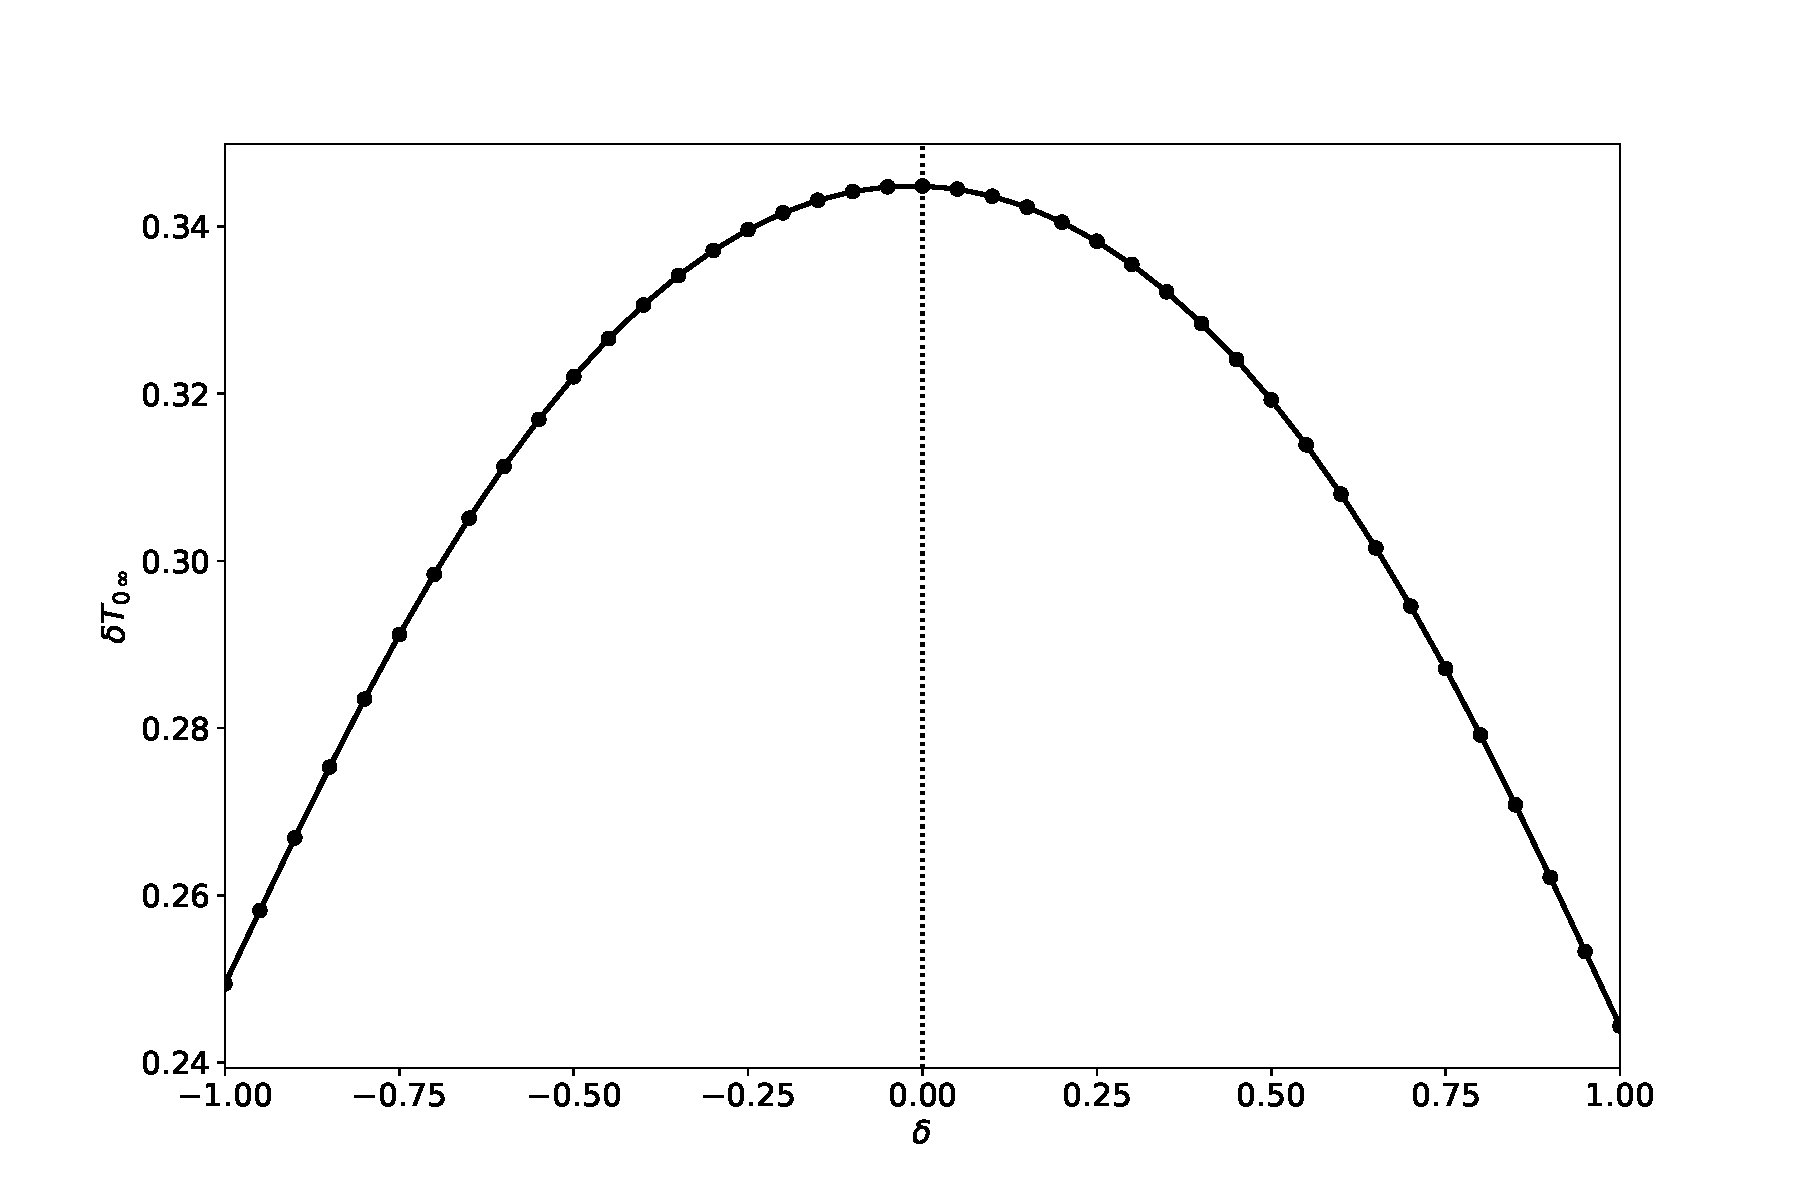
\includegraphics[width=\textwidth]{T0infty.pdf}}
\caption{The island temperature flattening parameter, $T_{0\,\infty}$, plotted as a function of the island asymmetry parameter, $\delta$.  \label{fig3}}
\end{figure}

\begin{figure}
\centerline{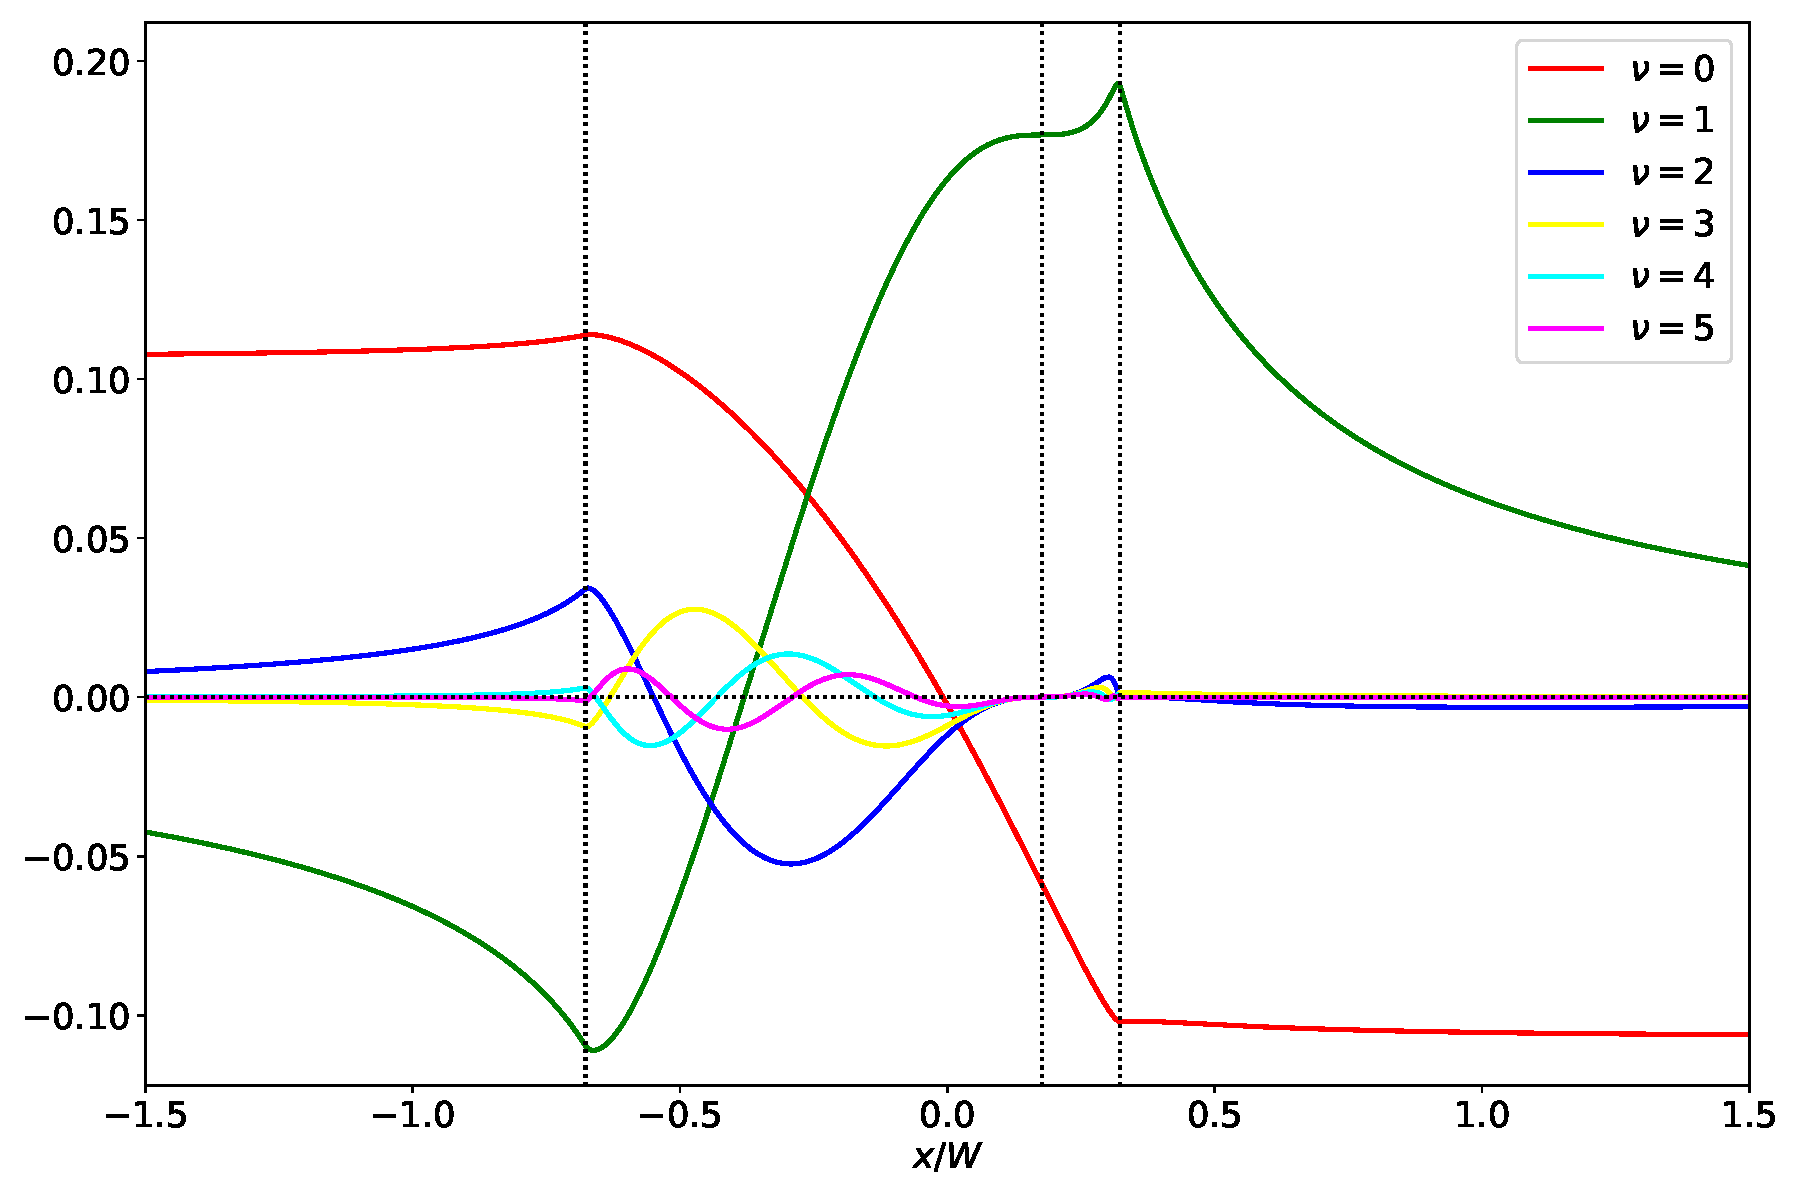
\includegraphics[width=\textwidth]{dTh.pdf}}
\caption{The helical harmonics of the normalized electron temperature  in the inner region, $\delta T_\nu(x/W)$, calculated for an asymmetric
magnetic island characterized by $\delta=0.5$.  The curve labelled $1$ actually
shows $\delta T_1(x/W) +  \delta/\sqrt{8}$. The vertical dotted lines show the locations of the inner limit of the magnetic separatrix,
the island X-point, and the outer limit of the magnetic separatrix, in order from the left to the right.\label{fig4}}
\end{figure}

\begin{figure}
\centerline{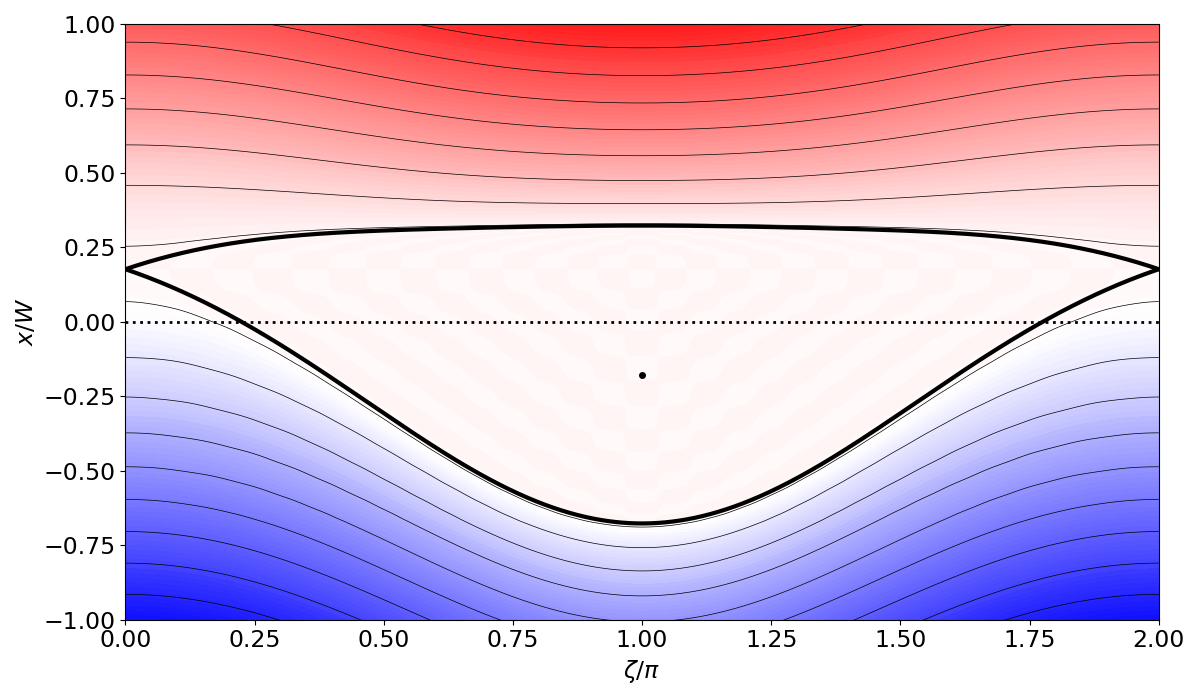
\includegraphics[width=\textwidth]{dTe.png}}
\caption{Contours of the normalized electron temperature profile, $\tilde{T}(x/W,\zeta)$, in the vicinity of an asymmetric magnetic island  characterized by
$\delta = 0.5$. The thick solid line shows the magnetic separatrix, the dotted line shows the rational surface, and the black dot shows the
island O-point.\label{fig5}}
\end{figure}

\end{document}